\documentclass[a4paper,12pt]{article}
\pagestyle{empty}
\usepackage{amsmath}
\usepackage{hyperref}
\usepackage[most]{tcolorbox}
\newcommand\numberthis{\addtocounter{equation}{1}\tag{\theequation}}
\begin{document}

\section*{Stopping Time}

\subsection*{Introduction}
Consider the question: given an object traveling at an initial velocity
$v_0$ toward a goal a distance $D$ away, a maximum acceleration of $a > 0$,
at what time $k$ should the object begin decelerating if it wants to
be at rest at the time it reaches object $D$, but (given this constraint),
it would like to reach object $D$ in the minimum time $f$.

\subsection*{General form of the Solution}

Since we would like to spend the minimum possible time reaching the object,
it follows that we should not decerate until the last possible moment $k$
which still allows us to come to rest at time $f$ and distance $D$ from
our starting point.

\begin{tcolorbox}
  Note: For particular combinations of initial conditions, it could be
  the case that the starting velocity is so great compared to the maximum
  acceleration that even if we begin the deceleration immediately,
  we still will not be at rest at the point in time after which we have
  travelled a distance $D$.
  If the object were to begin decelerating immediately, then it would
  take $v_0a$ time to come to a complete stop, meaning it would have
  traveled for a distance of $\frac{v_0^2}{2a}$, so as long as
  $D \geq \frac{v_0^2}{2a}$, we will find a valid, non-negative
  solution for $k$.
\end{tcolorbox}

\subsection*{Parameterized Equations of Motion}

Based on the General Form of the Solution, we can write down the
acceleration at every point in time as follows:

$$
  A(t) = \left\{
    \begin{array}{ll}
      0  & \mbox{if $t \leq k$} \\
      -a & \mbox{if $t > k$}
    \end{array}\\
  \right\}
$$

The plot in Figure 1 shows a rough example of a potential
velocity curve fitting the characteristics outlined above.

\begin{figure}[htbp]
\centering
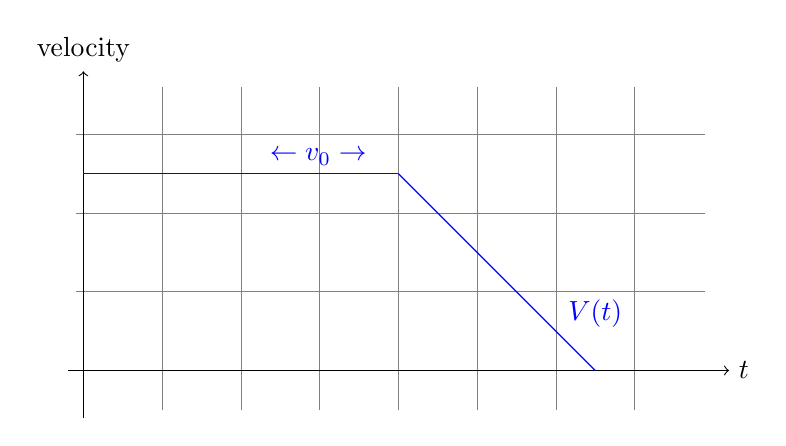
\begin{tikzpicture}[domain=0:4]
  \draw[very thin,color=gray] (-0.1,-0.5) grid (7.9,3.6);

  \draw[->] (-0.2,0) -- (8.2,0) node[right] {$t$};
  \draw[->] (0,-0.6) -- (0,3.8) node[above] {velocity};

  \draw[color=blue] plot (\x, 2.5) node[above=6pt, left=8pt] {$\leftarrow v_0 \rightarrow$};
  \draw[color=blue,domain=4.0:6.5] plot (\x, {-\x + 6.5}) node[above=12pt] {$V(t)$};
\end{tikzpicture}
\caption{Fig 1. A plot of the velocity over time.}
\label{fig:1}
\end{figure}

For a more complete example, see
\url{https://www.desmos.com/calculator/o8gxdsnxgw}.

Since acceleration is the derivative of velocity with respect to time, this
also allows us to deduce the velocity formula. We deduce the constants
using the boundary conditions $V(0) = V(k) = v_0$.

$$
  V(t) = \left\{
    \begin{array}{ll}
      v_0          & \mbox{if $t \leq k$} \\
      v_0 - a(t-k) & \mbox{if $t > k$}
    \end{array}
  \right\}
$$

Playing this trick once more, we can determine the position at every point in
time by integrating piecewise.  When $t \leq k$, we have:

\begin{align*}
  X_{t \leq k}(t) &= v_0 t + C_0 \\
  \intertext{Since $X_{t \leq k}(0) = 0$, $C_0=0$.}
  \intertext{When $t > k$:}
  X_{t > k}(t) &= v_0 t - \frac{a}{2} t^2 + akt + C_1 \\
  \intertext{We solve for $C_1$ by evaluating $X_{t > k}(f) = D$.}
  D = X_{t > k}(f) &= v_0 f - \frac{a}{2} f^2 + akf + C_1 \\
  C_1          &= D - (v_0 f - \frac{a}{2} f^2 + akf) \\
  \intertext{This gives the final equation for the position wrt time as:}
  X(t) &= \left\{
    \begin{array}{ll}
      v_0 t & \mbox{if $t \leq k$} \\
      - \frac{a}{2} t^2 + (v_0 + ak)t + \frac{a}{2} f^2 - (v_0 + ak) f + D & \mbox{if $t > k$}
    \end{array}
  \right\}
\end{align*}

Now let us use the fact that at time $t=f$ we will be at rest to express $f$ in
terms of $k$ and given values.

\begin{align*}
  V(f) = 0 &= v_0 - a(f - k) \\
 a(f - k)  &= v_0 \\
         f &= \frac{v_0}{a} + k \numberthis \label{eqn_for_f}
\end{align*}

\subsection*{Solving for k}

We know that the total distance travelled is $D$ and this
can be represented as the sum of two integrals.

\begin{align*}
  D &= \int_0^f V(t)dt \\
    &= \int_0^k V(t)dt + \int_k^f V(t)dt \\
  \intertext{For the first integral, the distance is $v_0k$ due to constant
  velocity.  For the second, since the deceleration is constant, the
  distance is half the distance as if the entire time was at speed $v_0$}
    &=  v_0k + \frac{(f-k)v_0}{2}
  \intertext{We can then substitute equation (1) and solve for $k$ directly}
  D &= v_0k + \left(\frac{v_0}{a} + k - k\right)\frac{v_0}{2} \\
  D &= v_0k + \frac{v_0^2}{2a} \\
  k &= \left(D - \frac{v_0^2}{2a}\right)/v_0
\end{align*}



\subsection*{Deprecated: Solving for k}

If we went forward with the method below, but plug in f
before expanding the terms incrorrectly, we'll see that 0=0.

True but not helpful.  Ignore the rest of the document.

Now we are ready to eliminate the stop time $f$ from the equation $X(t)$
using equation (1) above.

\begin{align*}
  X(t) &= \left\{
    \begin{array}{ll}
      v_0 t & \mbox{if $t \leq k$} \\
      - \frac{a}{2} t^2 + (v_0 + ak)t +
      \frac{a}{2} (\frac{v_0}{a} + k)^2 -
      (v_0 + ak)(\frac{v_0}{a} + k) + D & \mbox{if $t > k$}
    \end{array}
  \right\}
  \intertext{Expanding the $t>k$ branch in order to simplify}
  X_{t>k}(t) &= - \frac{a}{2} t^2 + (v_0 + ak)t +
  \frac{a}{2} \left(\frac{v_0^2}{a^2} + \frac{2v_0k}{a} + k^2\right)
  - \left(\frac{v_0^2}{a} + v_0k + v_0k + ak^2\right) + D \\
  X_{t>k}(t) &= - \frac{a}{2} t^2 + (v_0 + ak)t +
  \frac{v_0^2}{2a} + \frac{v_0k}{2} + \frac{k^2a}{2}
  - \frac{v_0^2}{a} - 2v_0k - ak^2 + D \\
  \intertext{}
  X_{t>k}(t) &= - \frac{a}{2} t^2 + (v_0 + ak)t
  - \frac{v_0^2}{2a} - \frac{3v_0k}{2} - \frac{k^2a}{2} + D \numberthis \label{eqn_f_elim}
\end{align*}

Finally we use the fact that from time $t=0$ to $t=f$, we cover a
distance of $D$, which is the definite integral of $V(t)$ over this time:

\begin{align*}
  D &= \int_0^f V(t)dt
  \intertext{Since $X(t)$ is the antiderivative of $V(t)$, we have:}
  D &= X(f) - X(0) \\
    &= X(f) - 0
  \intertext{Since $f > k$, we can use equation (2) to evaluate $X(t)$ at $f$}
  D &= - \frac{a}{2} f^2 + (v_0 + ak)f
       - \frac{v_0^2}{2a} - \frac{3v_0k}{2} - \frac{k^2a}{2} + D
       \numberthis \label{eqn_f_elim}
  \intertext{We will now substitute in equation (1) once more to eliminate these last $f$s}
  D &= - \frac{a}{2} (\frac{v_0}{a} + k)^2 + (v_0 + ak)(\frac{v_0}{a} + k)
       - \frac{v_0^2}{2a} - \frac{3v_0k}{2} - \frac{k^2a}{2} + D
  \intertext{Expand.}
  D &= - \frac{a}{2} \left(\frac{v_0^2}{a^2} + \frac{2v_0k}{a} + k^2\right)
    + \left(\frac{v_0^2}{a} + v_0k + v_0k + ak^2\right)
    - \frac{v_0^2}{2a} - \frac{3v_0k}{2} - \frac{k^2a}{2} + D
  \intertext{Distribute.}
  D &= -\frac{v_0^2}{2a} - v_0k - \frac{k^2a}{2}
       + \frac{v_0^2}{a} + 2v_0k + ak^2
       - \frac{v_0^2}{2a} - \frac{3v_0k}{2} - \frac{k^2a}{2} + D \\
  D &= -\frac{v_0^2}{2a} - v_0k - \frac{k^2a}{2}
       + \frac{v_0^2}{a} + 2v_0k + ak^2
       - \frac{v_0^2}{2a} - \frac{3v_0k}{2} - \frac{k^2a}{2} + D
  \intertext{Group like terms.}
  D &= k^2 (-\frac{a}{2} + a - \frac{a}{2})
    + k (-v_0 + 2v_0 - \frac{3v_0}{2})
    - \frac{v_0^2}{2a} + \frac{v_0^2}{a} - \frac{v_0^2}{2a} + D
  \intertext{We can now heavily simplify.}
  D &= k^2 (-\frac{a}{2} + a - \frac{a}{2})
    + k (-v_0 + 2v_0 - \frac{3v_0}{2})
    - \frac{v_0^2}{2a} + \frac{v_0^2}{a} - \frac{v_0^2}{2a} + D \\
  0 &= k^2 (a - a) - \frac{kv_0}{2} \\
  0 &= - \frac{kv_0}{2} \\
\end{align*}

\end{document}
